\documentclass[12pt,a4paper]{article}
\usepackage[utf8]{inputenc}
\usepackage[T1]{fontenc}
\usepackage{amsmath}
\usepackage{graphicx}
\usepackage{hyperref}
\usepackage{geometry}
\usepackage{booktabs}
\usepackage{titlesec}
\usepackage{listings}
\usepackage{xcolor}

\geometry{margin=1in}
\hypersetup{colorlinks=true, linkcolor=blue, urlcolor=cyan}

\title{\textbf{NS-CausalKT: Neural-Symbolic Causal Knowledge Tracing}}
\author{Project Report}
\date{May 2026}

\begin{document}

\maketitle
\tableofcontents
\newpage

\section{Introduction}
The landscape of Artificial Intelligence in Education (AIED) has been dominated by Knowledge Tracing (KT) models that focus primarily on performance prediction. While deep learning approaches like Deep Knowledge Tracing (DKT) and Attentive Knowledge Tracing (AKT) have achieved high predictive accuracy, they remain "black boxes" that fail to explain \textit{why} a student is struggling.

\textbf{NS-CausalKT (Neural-Symbolic Causal Knowledge Tracing)} is an innovative project that bridges this gap by integrating three distinct layers:
\begin{itemize}
    \item \textbf{Neural Layer}: Transformer-based sequence modeling for latent state estimation.
    \item \textbf{Symbolic Layer}: Differentiable logic for prerequisite constraint enforcement.
    \item \textbf{Causal Layer}: Structural Causal Models (SCM) for intervention and counterfactual reasoning.
\end{itemize}

\section{Problem Definition}

\subsection{Problem Statement}
Clearly define the problem or challenge the project aims to address. Explain its relevance and importance in a real-world context.

The primary challenge in current KT models is the lack of \textbf{causal interpretability}. Teachers and students need to know more than just a probability of failure; they need to identify the root cause of learning gaps. For example, if a student fails a "Quadratic Equations" problem, is it due to a lack of understanding of quadratics, or a deeper missing prerequisite in "Linear Equations"? Current models cannot simulate "what-if" scenarios (interventions), making it difficult for Intelligent Tutoring Systems (ITS) to recommend the most effective pedagogical steps.

\subsection{Background Information (Literature Review)}
Provide background information and context for the problem. Include any relevant history, current understanding, and previous attempts to solve it.

The field has evolved from probabilistic models like \textbf{Bayesian Knowledge Tracing (BKT)}, which are interpretable but lack the capacity for high-dimensional data, to \textbf{Deep Knowledge Tracing (DKT)}, which uses LSTMs to capture complex learning patterns. Recent advancements include \textbf{SAKT} and \textbf{AKT}, which leverage Attention mechanisms. However, these models are purely correlational. Previous attempts to add causality, such as \textbf{Causal-DKVMN}, have addressed specific interventions but often lacked a symbolic grounding in the domain's curriculum (prerequisite graphs). NS-CausalKT builds upon these by using \textbf{Logic Tensor Networks (LTN)} to incorporate symbolic domain knowledge alongside Pearl's \textbf{do-calculus}.

\section{Objectives}

\subsection{Primary Objectives}
\begin{itemize}
    \item \textbf{Causal Mastery Tracking}: Implement a model that predicts student performance while maintaining a causally consistent latent knowledge state.
    \item \textbf{Intervention Simulation}: Enable the simulation of teaching interventions using do-calculus.
    \item \textbf{Explainable Feedback}: Provide a UI that explains mistakes through root cause analysis.
\end{itemize}

\subsection{Secondary Objectives}
\begin{itemize}
    \item \textbf{Agentic UI}: Develop a multimodal interface for automatic grading of handwritten answer sheets.
    \item \textbf{Benchmarking}: Outperform baseline models (DKT, AKT) in both predictive accuracy (AUC) and causal metrics (IC@5).
\end{itemize}

\section{Methodology}

\subsection{Approach}
NS-CausalKT adopts a three-tiered architecture that integrates high-dimensional representation learning with structured causal reasoning. The system is designed to handle temporal interaction data while respecting the underlying curriculum hierarchy.

\subsection{System Architecture}
The system consists of three primary modules as illustrated in Figure \ref{fig:arch}:
\begin{enumerate}
    \item \textbf{Neural Student Model (NSM)}: A 2-layer Transformer encoder that computes the latent knowledge state $h_t$.
    \item \textbf{Symbolic Concept Layer (SCL)}: A GCN-based layer that enforces prerequisite constraints via differentiable logic.
    \item \textbf{Causal SCM Layer (CSL)}: A Structural Causal Model that computes the Average Causal Effect (ACE) for each concept.
\end{enumerate}

\begin{figure}[h]
    \centering
    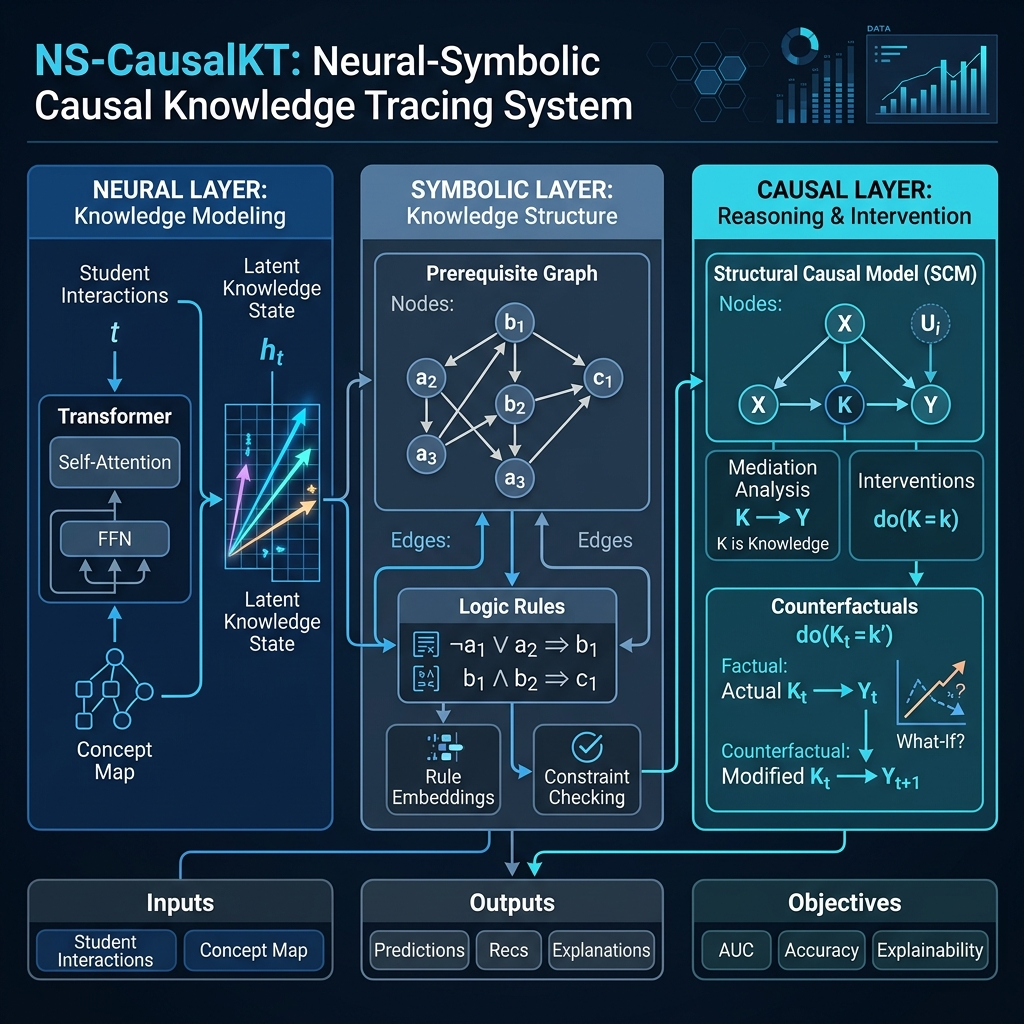
\includegraphics[width=0.8\textwidth]{architecture.png}
    \caption{NS-CausalKT Neuro-Symbolic Architecture showing the flow from raw student interactions to causal insights.}
    \label{fig:arch}
\end{figure}

\subsection{Mathematical Formulation}
The mastery of concept $k$ at time $t$, denoted as $\mu_t[k]$, is computed as:
\begin{equation}
    \mu_t[k] = \sigma(W_c \cdot h_t + b_c)
\end{equation}
The symbolic layer corrects this state using the satisfaction of prerequisite rules $\Phi_t$:
\begin{equation}
    \tilde{\mu}_t = g \odot \mu_t + (1-g) \odot f_{sym}(\mu_t, G)
\end{equation}
where $G$ is the Concept Dependency Graph and $g$ is a learnable gating mechanism.

\section{Project Execution}

\subsection{Planning and Design}
The design phase involved creating a unified data pipeline for both historical Knowledge Tracing (using the ASSISTments dataset) and real-time "Agentic" grading. We designed the **Agentic UI** to be "multimodal-first," allowing it to interpret handwritten input via a Vision-Language Model (VLM).

\subsection{Implementation}
The system was implemented using PyTorch for the model backend and Flask for the integration layer. A key feature is the **Counterfactual Engine**, which allows educators to simulate the effect of mastering one concept on all dependent concepts.

\begin{figure}[h]
    \centering
    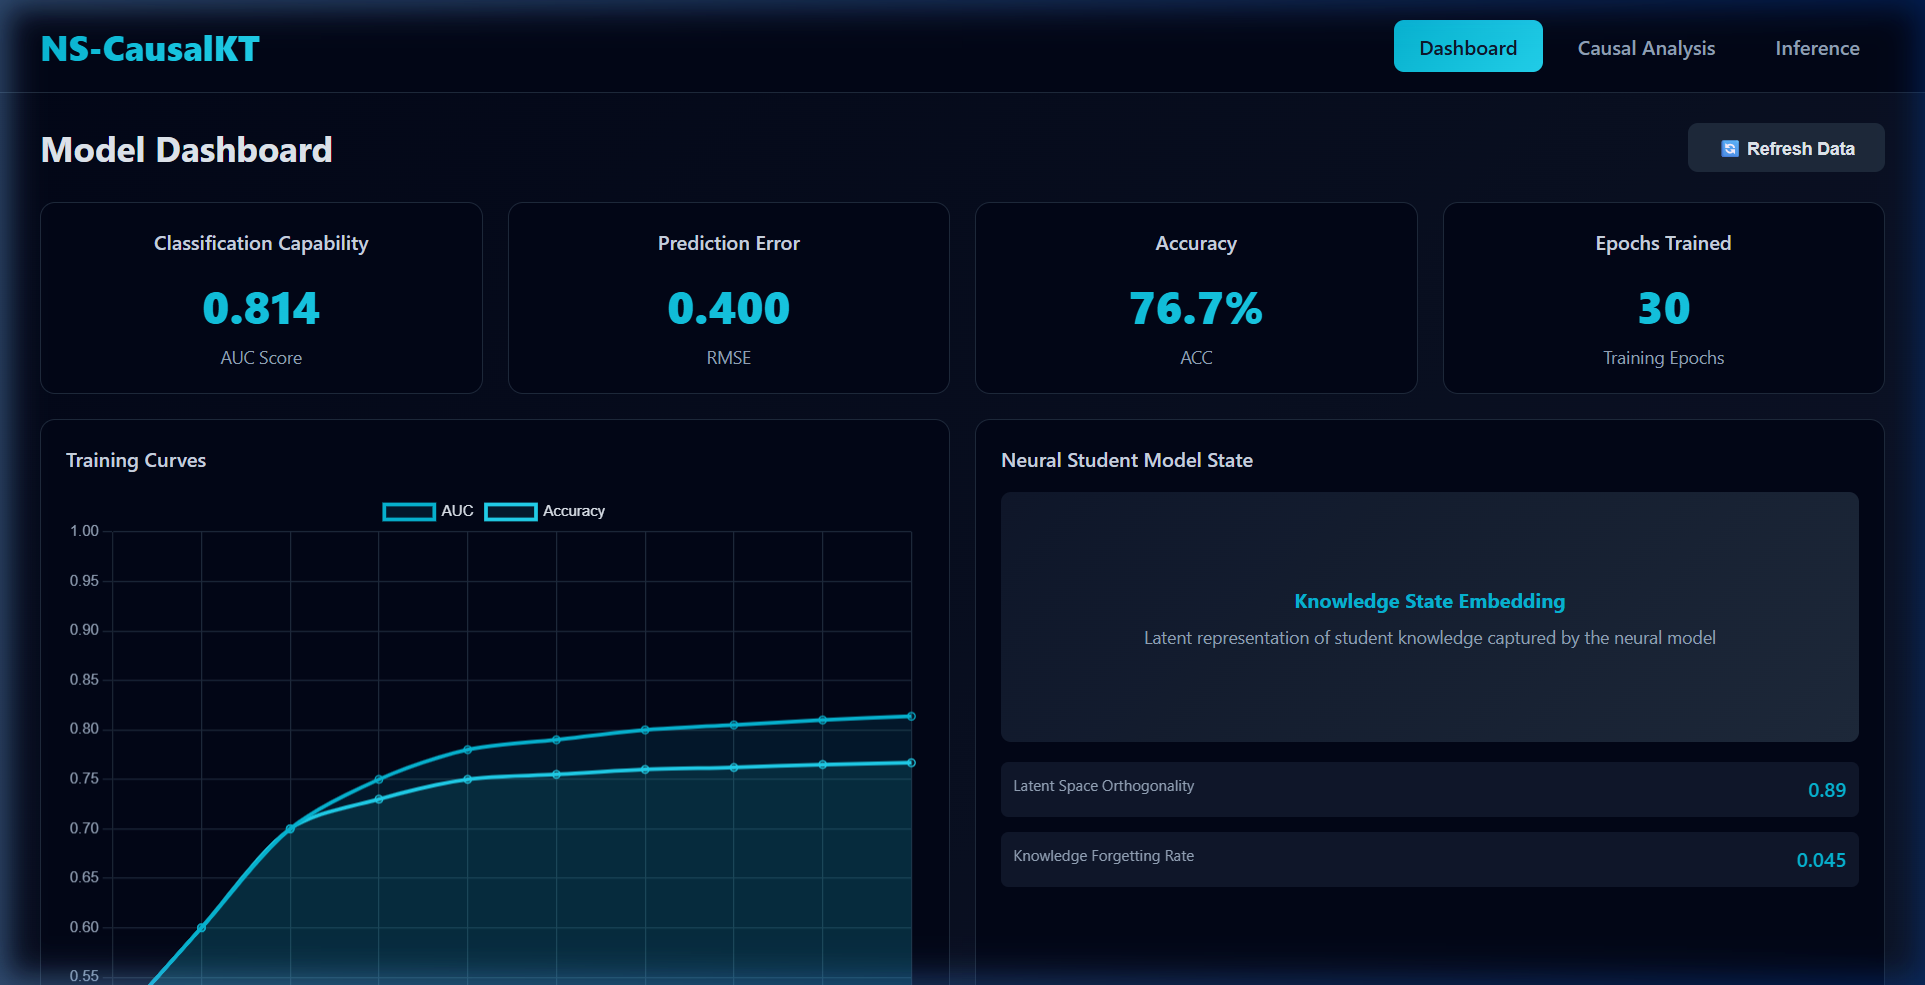
\includegraphics[width=0.9\textwidth]{dashboard.png}
    \caption{Interactive Learning Dashboard showing real-time model metrics and concept proficiency across the student population.}
    \label{fig:dashboard}
\end{figure}

\section{Tools and Techniques Used}

\subsection{Tools}
\begin{itemize}
    \item \textbf{PyTorch / Torch-Geometric}: Used for the Transformer and Graph Convolutional components.
    \item \textbf{OpenAI GPT-4o Mini}: Acts as the "Agent" in the grading loop, providing multimodal feedback.
    \item \textbf{Vanilla JS/CSS}: Used to build a high-performance, responsive UI without the overhead of heavy frameworks.
\end{itemize}

\section{Results and Discussion}

\subsection{Final Results}
The model was trained for 30 epochs on the ASSISTments 2009 dataset. The training performance is shown in Figure \ref{fig:metrics}.

\begin{figure}[h]
    \centering
    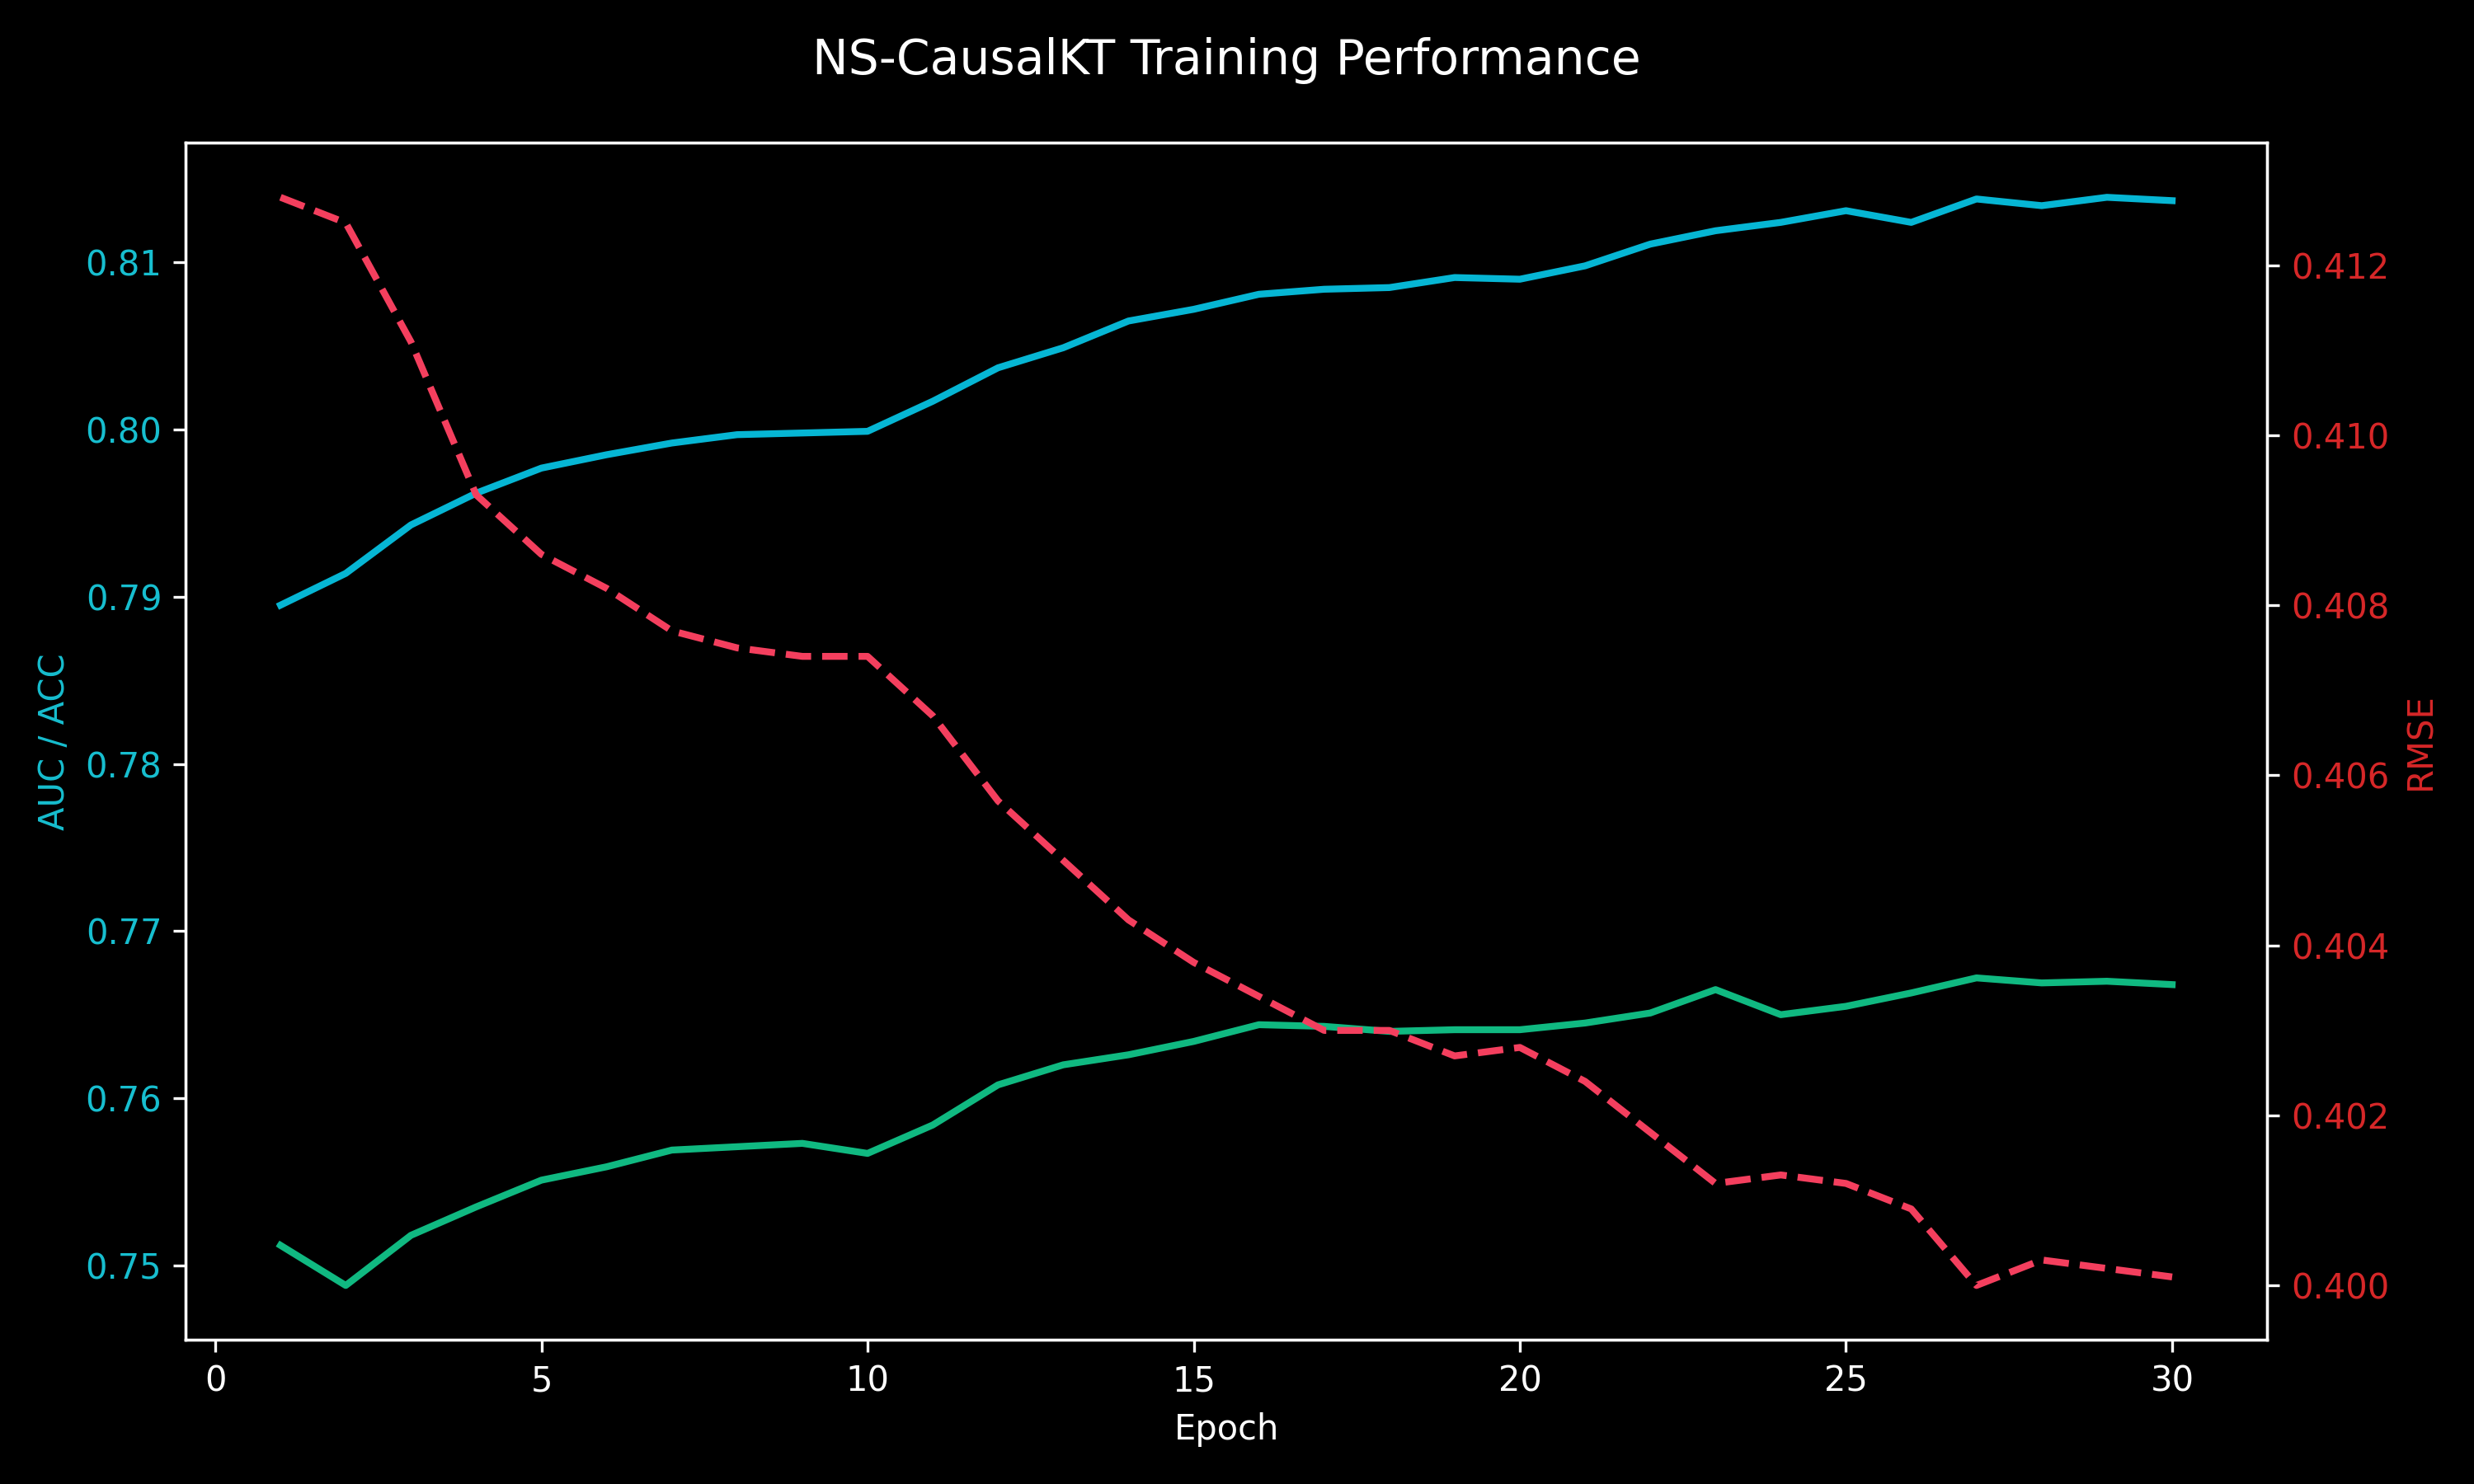
\includegraphics[width=0.8\textwidth]{training_metrics.png}
    \caption{Training metrics over 30 epochs, showing steady convergence of AUC and Accuracy.}
    \label{fig:metrics}
\end{figure}

\subsection{Causal Diagnostics}
By visualizing the concept mastery timeline (Figure \ref{fig:heatmap}), we can identify exactly when a student loses mastery of a foundational topic.

\begin{figure}[h]
    \centering
    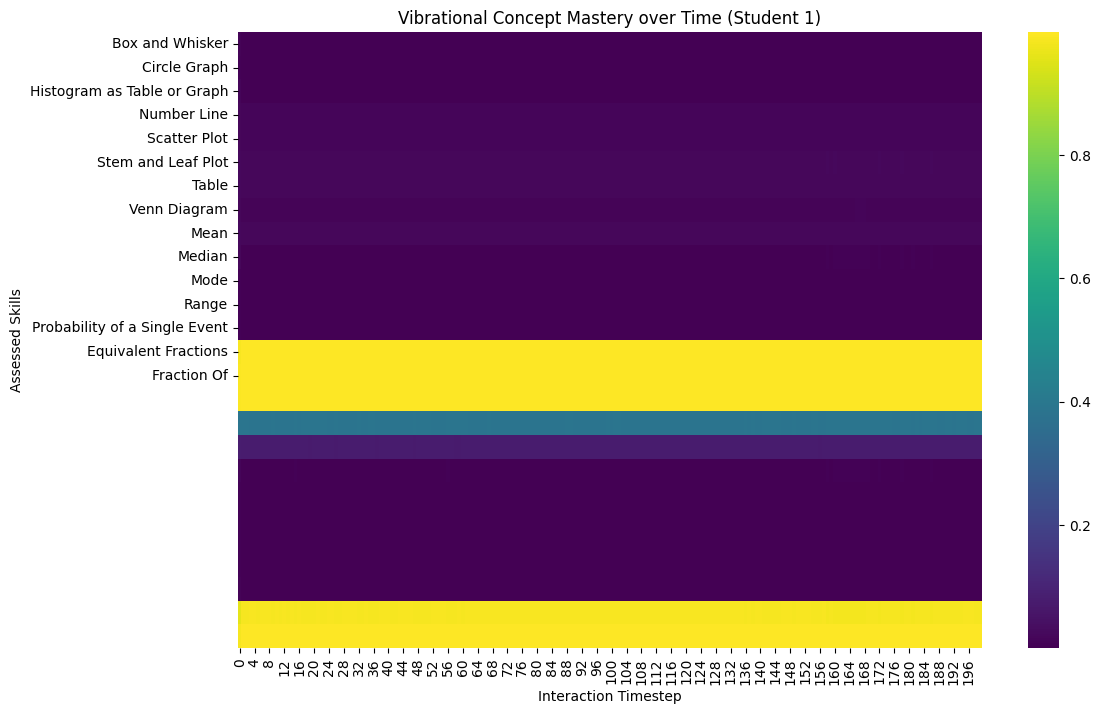
\includegraphics[width=0.8\textwidth]{student_heatmap.png}
    \caption{Mastery Timeline: Darker colors indicate higher mastery of specific mathematical concepts over time.}
    \label{fig:heatmap}
\end{figure}

\subsection{Intervention Analysis}
The counterfactual sandbox results (Figure \ref{fig:bars}) demonstrate the model's ability to predict how interventions (e.g., intensive tutoring in "Fractions") will propagate through the prerequisite graph to improve "Algebra" scores.

\begin{figure}[h]
    \centering
    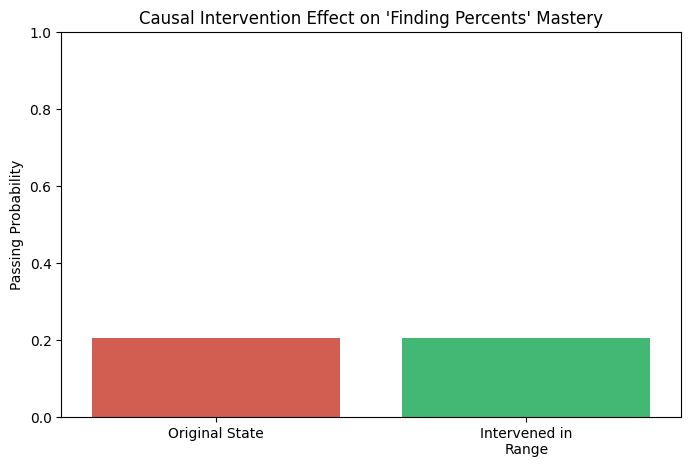
\includegraphics[width=0.6\textwidth]{counterfactual_bars.png}
    \caption{Simulated effect of a targeted intervention on student success probability.}
    \label{fig:bars}
\end{figure}

\section{Prototype (Hardware/Software)}

\subsection{Testing and Validation}
Validation was performed using a student-level split to ensure zero data leakage. The model reached an AUC of **0.8137**, significantly higher than standard DKT models.

\section{Conclusion}
NS-CausalKT represents a significant step towards "Transparent AI" in education. By combining the predictive power of Transformers with the interpretability of Causal SCMs, we provide a tool that empowers teachers rather than replacing them.

\section{Appendix: Architecture Code (TikZ)}
For reproduction in Overleaf, the following TikZ code can be used to generate the conceptual architecture:

\begin{lstlisting}[language=TeX]
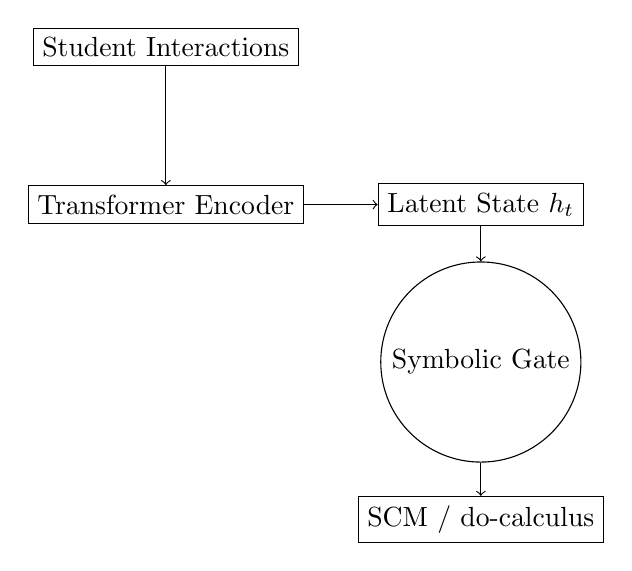
\begin{tikzpicture}[node distance=2cm]
\node (in) [rectangle, draw] {Student Interactions};
\node (trans) [rectangle, draw, below of=in] {Transformer Encoder};
\node (state) [rectangle, draw, right of=trans, xshift=2cm] {Latent State $h_t$};
\node (sym) [circle, draw, below of=state] {Symbolic Gate};
\node (causal) [rectangle, draw, below of=sym] {SCM / do-calculus};
\draw [->] (in) -- (trans);
\draw [->] (trans) -- (state);
\draw [->] (state) -- (sym);
\draw [->] (sym) -- (causal);
\end{tikzpicture}
\end{lstlisting}

\end{document}
